%% Lab Report for EEET2493_labreport_template.tex
%% V1.0
%% 2019/01/16
%% This is the template for a Lab report following an IEEE paper. Modified by Francisco Tovar after Michael Sheel original document.


%% This is a skeleton file demonstrating the use of IEEEtran.cls
%% (requires IEEEtran.cls version 1.8b or later) with an IEEE
%% journal paper.
%%
%% Support sites:
%% http://www.michaelshell.org/tex/ieeetran/
%% http://www.ctan.org/pkg/ieeetran
%% and
%% http://www.ieee.org/

%%*************************************************************************
%% Legal Notice:
%% This code is offered as-is without any warranty either expressed or
%% implied; without even the implied warranty of MERCHANTABILITY or
%% FITNESS FOR A PARTICULAR PURPOSE! 
%% User assumes all risk.
%% In no event shall the IEEE or any contributor to this code be liable for
%% any damages or losses, including, but not limited to, incidental,
%% consequential, or any other damages, resulting from the use or misuse
%% of any information contained here.
%%
%% All comments are the opinions of their respective authors and are not
%% necessarily endorsed by the IEEE.
%%
%% This work is distributed under the LaTeX Project Public License (LPPL)
%% ( http://www.latex-project.org/ ) version 1.3, and may be freely used,
%% distributed and modified. A copy of the LPPL, version 1.3, is included
%% in the base LaTeX documentation of all distributions of LaTeX released
%% 2003/12/01 or later.
%% Retain all contribution notices and credits.
%% ** Modified files should be clearly indicated as such, including  **
%% ** renaming them and changing author support contact information. **
%%*************************************************************************

% \subsection{Goals}
The research objective is to build a certified Reduced Order Model (ROM) 
for a nonlinear Burgers-like parametrized unsteady PDE, 
within a one-dimensional moving boundary.
The main body of the PDE, 
the geometrical definition of the moving boundary,
and the boundary conditions will be parametrized.

The main task at hand is to be able to create a reduced order model 
not only efficiently,
but skipping the Jacobian transformation.
Such transformation is usually required in the context of moving meshes,
and sometimes it may not even be explicitly available.

Additionally, this could potentially allow us to use our reduction scheme with existing codebases,
provided that we can access the operators and some of their entries. 

% We aim at providing a concise description of the reducing procedure, 
% a posteriori error estimators to certify their use and 
% a numerical example to showcase computational costs and implementation details.
\subsection{Research Questions}
Of particular interest will be the reduction of the nonlinear term.
We will discuss how the approximation error of this term interacts with 
the approximation error of the remaining operators and the reduced basis itself.
Two techniques to reduce the nonlinear will be compared and discussed.
One approach is to collect the nonlinear operator snapshots as the FOM is integrated;
the other one is to collect the snapshots from evaluations of the nonlinear operator
using the reduced basis elements 
(after all, the solution is a linear combinations of the latter). 
These two methods could potentially produce different bases, 
with different approximation errors. 

Regarding the movement of the mesh, two types of movements will be analyzed.
First, the natural oscillation of the moving piston.
This movement spreads out evenly the stretching among the cells, 
removing the spatial dependency from the Jacobian.
Then, a nonlinear mesh movement will be introduced, 
with the concentration of nodes around specific regions as time changes.
These regions will be user-defined, not solution dependent.
Our aim is to mimick the effects of shock tracking or mesh refinement techniques, 
without explicitly using them, to prove the good working of the reduction
method, in isolation from specific applications. 

The certification of the HROM will be done with a model truncation technique.
This is a standard approach, useful due to its generality.

All in all, we intend to exercise in a one-dimensional domain
the different techniques we will be using;
knowing that since our approach is purely algebraic, 
it would translate naturally to higher dimensions,
albeit more involved codebase implementations details and costs.

% Because the ROM can approach arbitrarily close the FOM, 
% one would like to have a rough idea of how many reduced basis will be required to attain such accuracy. 
% To that end, bounds for convergence rates of the reduction procedures must be obtained, 
% and a posteriori error estimates of the reduction model to certify the solution stayed within the desired bracket. 

% The numerical implementation will be validated with the manufactured solutions method.

\subsection{Scope}
The project is mainly practice-oriented, in that we shall design, 
build and evaluate the procedure to construct the HROM.
We will use known theoretical results 
to guide our assessment of the reduction technique, 
but we do not expect to formulate new ones.

\begin{figure}[h]
   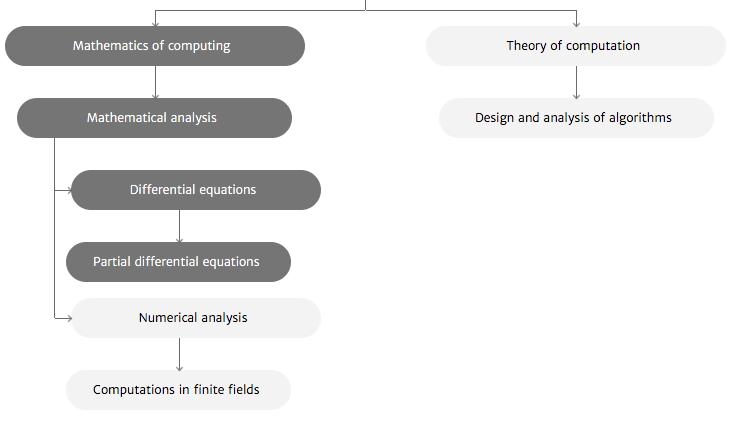
\includegraphics[width=\columnwidth]{research_project/figures/index.png}
   \caption{Conceptual location of the M. Sc. Thesis project.}
\end{figure}

% Nevertheless, we intend to have theoretical content too, as convergence rates 
% and a posteriori error estimates require the deployment of theoretical development and theorems\footnote{
%    Which rely on the usual stability factors and arguments present in the Finite Element body.} 
% to find sharp bounds.

% \subsection{Implementation of the Moving Domain}
% To capture the effects of a moving domain without unnecessarily complicating the implementation, 
% we shall assume a separable deformation across the mesh, 
% \begin{equation}
%    \vec{d}(t;\mu) = g(t) \vec{d}_s(\mu),
% \end{equation}
% where the spatial deformation $\vec{d}_s(\mu)$ will be obtained from the solution 
% of a simple Laplace problem over an initial undeformed domain $\Omega_0$,
% \begin{align*}
%    -\Delta \vec{d}_s &= \vec{0}, \quad \vec{x} \in \Omega_0, \\
%    \vec{d}_s &= \vec{h}(\vec{x}, \mu) \in \partial\Omega_0.
% \end{align*}
% In this way, we obtain a smooth displacement across the domain, 
% due to the harmonic properties of the Laplacian operator. 

% For industrial applications, the elasticity equation ought to be solved instead, 
% but this would only add complications to our problem which are out of scope for the reduction process we are concerned with.

% This problem can be reduced too at the beginning of the offline phase, 
% so that quicker displacements are obtained during the solution of the main PDE. 
% The reduction technique for this problem is simpler, 
% as it does not depend on time thanks to the separation assumption. 

% By introducing the construction of a posteriori error estimators, 
% one can certify the results of the reduced basis for unseen in the training phase parameters.

%% Theory-oriented
% Theory development
% Theory testing

%% Practice-oriented: intervention cycle
% Problem Analysis
% Diagnosis
% Design
% Change
% Evaluation


%% Research Strategy
% Suitability
% Duration
% Feasibility

% \subsection{Conclusions}
% \label{sec:conclusions}
% The conclusion of this thesis will establish the reduction procedure for parametrized unsteady PDEs with a moving mesh.

% Thanks to the a posteriori error estimates, the procedure will be certified.
% That is, the error between the FOM and the ROM will be proved to be under a given threshold.

